\documentclass[letter,12pt]{article}
\usepackage[left=2.54cm, right=2.54cm, top=2.54cm, bottom=2.54cm]{geometry} % Márgenes APA
\usepackage{setspace} % Interlineado
\setlength{\parindent}{1.27cm} % Sangría estándar APA
\setlength{\parskip}{0pt}     % Sin espacio entre párrafos
\usepackage{graphicx} % Para insertar imágenes
\usepackage{float} % Para posicionar imágenes y tablas
\usepackage{caption} % Para modificar captions de tablas e imágenes
\usepackage{csquotes} % Para mejor manejo de citas
\usepackage{amsmath} % Para ecuaciones matemáticas
\usepackage{svg}
\usepackage{indentfirst}
\usepackage[utf8]{inputenc} % Soporte para UTF-8
\usepackage[T1]{fontenc}    % Codificación de fuente
\usepackage{textcomp}       % Símbolos adicionales (≈)
\usepackage{tabularx} % <-- Añadir al preámbulo si no está
\usepackage{longtable} % Añadir al preámbulo si no está
% \usepackage{ltablex} % Añadir al preámbulo si no está
% \keepXColumns % Para que X funcione igual que en tabularx

\usepackage{algorithm}
\usepackage{algorithmic}

\usepackage{listings}
\usepackage{xcolor}

\lstset{
	language=C,
	basicstyle=\ttfamily\small,
	keywordstyle=\color{blue},
	commentstyle=\color{gray},
	stringstyle=\color{orange},
	numbers=left,
	numberstyle=\tiny\color{gray},
	stepnumber=1,
	frame=single,
	breaklines=true
}


%==========REFERENCIAS=============
\usepackage[backend=bibtex,style=ieee,language=spanish]{biblatex}
\addbibresource{referencias.bib}

\usepackage[
    pdftitle={Tarea \# 2 - Modelado de sistemas}, % Título del PDF
    pdfauthor={Barquero, J., Feng, J., Montero, A.},   % Autor del PDF
    pdfsubject={CE1110 - Análisis de Señales Mixtas}, % Tema del PDF
    pdfkeywords={}, % Palabras clave del PDF
    pdfproducer={LaTeX with hyperref package},
    pdfcreator={pdfLatex}
]{hyperref}

\hypersetup{
    colorlinks=true,        % Colorea los enlaces en lugar de usar cajas alrededor de ellos
    linkcolor = black,
    urlcolor  = blue,
    citecolor = black,
    anchorcolor = blue         % Color de los enlaces externos
}

\begin{document}
% ====== Portada ======
\begin{titlepage}
    \centering
    {\LARGE \textbf{Tarea \# 2} \par}
    {\LARGE Modelado de sistemas \par}
    \vspace{1.5cm}
    {\large José Bernardo Barquero Bonilla \\ 2023150476 \par}
    {\large Jimmy Feng Feng \\ 2023060347 \par}
    {\large Alexander Montero Vargas \\ 2023166058 \par}
    \vspace{1.5cm}
    {\Large Instituto Tecnológico de Costa Rica \par}
    {\large Escuela de Ingeniería en Computadores \par}
    {\large Curso: CE1110 - Análisis de Señales Mixtas \par}
    \vspace{1.5cm}
    {\large Profesor: Luis Alberto Chavarría Zamora \par}
    \vfill
    {\large 23 de Noviembre de 2025 \par}
\end{titlepage}

% ====== Desarrollo ======

% ====== Pregunta 1 ======
\section{Respuesta al impulso y al escalón en sistemas}

\par La respuesta al impulso y al escalón son importantes porque describen el comportamiento completo de un sistema:

\begin{itemize}
	\item \textbf{Respuesta al impulso:} Denotada como $h(t)$ en tiempo continuo, se define como la salida de un sistema cuando la entrada es un impulso unitario $\delta(t)$. Para un sistema LTI, la respuesta total del sistema ante cualquier entrada $x(t)$ puede calcularse mediante la operación de convolución \cite{oppenheim1997signals}:
	
	\begin{equation}
		y(t) = x(t) * h(t) = \int_{-\infty}^{\infty} x(\tau)h(t-\tau) d\tau
	\end{equation}
	
	
	\item \textbf{Respuesta al escalón:} Es la salida cuando la entrada es el escalón unitario $u(t)$. Se obtiene como la convolución del escalón con la respuesta al impulso\cite{oppenheim1997signals}:
	
	\begin{equation}
		s(t) = u(t) * h(t) = \int_{-\infty}^{t}h(\tau)d\tau
	\end{equation}
	
\end{itemize}

\par En el caso de los sistemas LTI, la respuesta al impulso caracteriza completamente al sistema desde el punto de vista entrada-salida. Es decir, 
conociendo $h(t)$, se puede predecir la salida del sistema para cualquier señal de entrada 
mediante la operación de convolución. Esto constituye una de las bases del análisis de sistemas 
establecida en la teoría de señales y sistemas.\cite{oppenheim1997signals}



% ====== Pregunta 2 ======
\section{Frecuencia de muestreo del sistemas de control continuo}

En sistemas de control digital, la elección de la frecuencia de muestreo no es arbitraria, sino que depende directamente de la dinámica de la planta. En particular, esta frecuencia debe ser lo suficientemente alta para capturar adecuadamente el comportamiento del sistema continuo, evitando distorsiones significativas debidas al proceso de discretización.

Una regla práctica ampliamente aceptada en control digital establece que la frecuencia de muestreo $f_s$ debe ser varias veces mayor que el ancho de banda del sistema, o en su defecto, mayor que su frecuencia dominante. Matemáticamente, esta recomendación se expresa como \cite{LandauDigitalControl}:

\begin{equation}
	f_s = k \cdot f_{B}, \quad \text{donde } k \in [6,\,25]
\end{equation}

donde:
\begin{itemize}
	\item $f_s$ es la frecuencia de muestreo
	
	\item $f_{B}$ es el ancho de banda del sistema (planta)
	
	\item $k$ es un factor adimensional que depende del compromiso entre precisión y complejidad computacional
\end{itemize}

De acuerdo con valores típicos utilizados en sistemas de control digital, los \textit{servo-mecanismos} se caracterizan por poseer dinámicas relativamente rápidas, por lo que requieren períodos de muestreo pequeños para capturar adecuadamente su comportamiento. 

Según tablas de referencia para sistemas de control industrial, el período de muestreo recomendado para servo-mecanismos se encuentra en el rango \cite{LandauDigitalControl}:

\begin{equation*}
	T_s \in [0.001,\;0.05] \;\text{s}
\end{equation*}

lo que equivale a una frecuencia de muestreo entre:

\begin{equation*}
	f_s \in [20,\;1000] \;\text{Hz}.
\end{equation*}

% ====== Pregunta 3 ======
\section{PID en microcontrolador}

En control continuo, el PID se expresa como:

\begin{equation}
	u(t) = K_p e(t) + K_i \int_{0}^{t} e(\tau)\, d\tau + K_d \frac{de(t)}{dt}
	\label{eq:pid_continuo}
\end{equation}

En un microcontrolador, se implementa en forma discreta, debido al uso de señales muestreadas con un periodo de muestreo $T_s$. Una forma discreta del PID es \cite{OchoaPIDDigital}:

\begin{equation}
	u[k] = K_p e[k] 
	+ K_i \sum_{i=0}^{k} e[i]\,T_s 
	+ K_d \frac{e[k] - e[k-1]}{T_s}
	\label{eq:pid_discreto}
\end{equation}

donde:
\begin{itemize}
	\item $e[k]$ es el error en el instante $k$,
	\item $T_s$ es el período de muestreo,
	\item $u[k]$ es la salida de control,
	\item $K_p$, $K_i$ y $K_d$ son las constantes proporcional, integral y derivativa.
\end{itemize}

Para la implementación digital, el cálculo del control se realiza en cada interrupción generada por un temporizador con período $T_s$, actualizando el error, el término integral acumulado y el término derivativo.

No se utiliza la función $delay()$ debido a bloquea la ejecución del programa. \cite{ArduinoDelay} Esto afecta el desempeño del PID porque el muestro deja de ser uniforme. Como alternativa, se utiliza interrupcciones con la función $interrupts()$.

Las interrupciones permiten que el microcontrolador responda a eventos externos en segundo plano sin detener el programa principal. \cite{ArduinoInterrupts}

\begin{algorithm}[H]
	\caption{Algoritmo PID Discreto en Microcontrolador}
	\begin{algorithmic}[1]
		
		\REQUIRE $K_p, K_i, K_d$, período de muestreo $T_s$, referencia $r[k]$, medida $y[k]$
		\ENSURE Señal de control $u[k]$
		
		\STATE Inicializar $e_{prev} \gets 0$
		\STATE Inicializar $I \gets 0$
		
		\WHILE{el sistema esté en ejecución}
		
		\STATE Medir salida del sistema $y[k]$
		\STATE Calcular error: $e[k] \gets r[k] - y[k]$
		
		\STATE Calcular término integral:
		\[
		I \gets I + e[k] \cdot T_s
		\]
		
		\STATE Calcular término derivativo:
		\[
		D \gets \frac{e[k] - e_{prev}}{T_s}
		\]
		
		\STATE Calcular señal de control:
		\[
		u[k] \gets K_p e[k] + K_i I + K_d D
		\]
		
		\STATE Actualizar error anterior:
		\[
		e_{prev} \gets e[k]
		\]
		
		\STATE Aplicar $u[k]$ al actuador
		
		\STATE Esperar interrupción del temporizador (periodo $T_s$)
		
		\ENDWHILE
		
	\end{algorithmic}
\end{algorithm}


% ====== Pregunta 4 ======
\section{Diagrama de bloques del sistema}

El sistema desarrollado corresponde a un sistema de control en lazo cerrado para una puerta corrediza accionada mediante un motor de corriente directa (DC). Su objetivo es regular la velocidad de desplazamiento de la puerta ante tres niveles de velocidad seleccionables por el usuario.

% ===== Figura 1 =====
\begin{figure}[H]
	\centering
	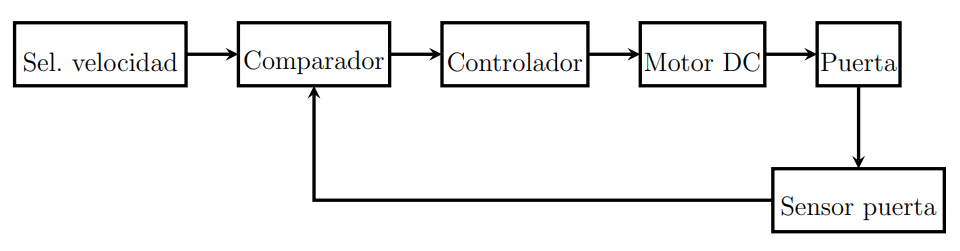
\includegraphics[width=13cm]{Media/diagrama_bloques.png}
	\caption{Diagrama de bloques del sistema}
	\label{fig:diagrama_bloques}
\end{figure}

En la figura \ref{fig:diagrama_bloques} se muestra el diagrama de bloques del sistema. Este sistema está compuesto por bloques tanto continuos como discretos, los cuales interactúan entre sí para lograr el control adecuado de la planta. A continuación se describe detalladamente cada uno de sus componentes.

\subsection{Selector de velocidad}

El selector de velocidad permite al usuario escoger entre tres valores discretos de velocidad de desplazamiento de la puerta (por ejemplo: baja, media y alta). Este bloque se implementa de forma discreta mediante botones físicos o interruptores conectados al microcontrolador.  

Cada opción corresponde a un valor de referencia $r[k]$, que es convertido a una magnitud compatible con el sistema de control, por ejemplo, una velocidad angular deseada en rad/s. 

Este bloque es de naturaleza discreta, ya que conmuta entre niveles predefinidos.

\subsection{Comparador}

El comparador se encarga de calcular el error del sistema, como la diferencia entre la referencia seleccionada y la señal medida por el sensor:

\begin{equation}
	e[k] = r[k] - y[k]
\end{equation}

donde:
\begin{itemize}
	\item $r[k]$ es la velocidad de referencia seleccionada por el usuario
	\item $y[k]$ es la velocidad real medida del sistema
	\item $e[k]$ es el error de control
\end{itemize}

Este bloque se implementa en forma discreta dentro del microcontrolador, ya que opera sobre valores muestreados.

\subsection{Controlador PID digital}

El controlador corresponde a un PID digital implementado en el microcontrolador. Este recibe el error $e[k]$ y calcula la señal de control $u[k]$ que se envía al actuador.

Su ecuación general está dada por la ecuación \ref{eq:pid_discreto}.

Este bloque es completamente discreto debido a que trabaja con señales muestreadas y opera en intervalos de tiempo $T_s$, generados por interrupciones de temporizador en el microcontrolador.

Además, el controlador dispone de un modo de operación conmutado:
\begin{itemize}
	\item \textbf{Modo activado}: el controlador regula automáticamente la velocidad del motor.
	\item \textbf{Modo desactivado}: el motor opera sin control, para observar el comportamiento del sistema en lazo abierto.
\end{itemize}

\subsection{Motor de corriente directa (Planta)}

El motor DC es el actuador principal del sistema y se encarga de convertir la señal de control eléctrica $u[k]$, en forma de PWM, en movimiento rotacional.

\subsection{Puerta corrediza}

La puerta representa la carga mecánica conectada al eje del motor, la cual se desplaza sobre un riel lineal. Este bloque transforma el movimiento rotacional del motor en un movimiento lineal de traslación.

Este sistema es de naturaleza continua, ya que su movimiento ocurre en tiempo real y de forma permanente, dependiendo de las fuerzas aplicadas y las inercias involucradas.

\subsection{Sensor de posición o velocidad}

El sensor es el encargado de medir el estado actual de la puerta o del motor, ya sea en términos de posición lineal o velocidad angular.  

Puede tratarse de:
\begin{itemize}
	\item Un sensor óptico
	\item Un potenciómetro lineal
	\item Sensores magnéticos
\end{itemize}

\subsection{Sistema de realimentación}

Finalmente, la señal medida $y[k]$ se realimenta hacia el comparador, cerrando el lazo de control.  
Este esquema permite:
\begin{itemize}
	\item Compensar perturbaciones externas
	\item Corregir errores de velocidad
	\item Mantener la velocidad deseada a pesar de variaciones en la carga
\end{itemize}

% ====== Pregunta 5 ======
\section{Modelo matemático y respuesta de la planta}


\subsection{Modelos matemáticos en dominio del tiempo}

El modelo de un motor DC se obtiene a partir de sus ecuaciones eléctrica y mecánica.


La ecuación del modelo eléctrico es:

\begin{equation}
	v(t) = Ri(t) + L \frac{di(t)}{dt} + k_b\omega(t)
	\label{eq:mod_elec}
\end{equation}

donde $v(t)$ es el voltaje aplicado a la armadura, $i(t)$ es la corriente, $R$ y $L$ son la resistencia e inductancia de la armadura, y $k_b$ es la constante de fuerza contraelectromotriz.


La ecuación del modelo mecánico es:

\begin{equation}
	k_mi(t) = J \frac{d\omega(t)}{dt} + B\omega(t)
	\label{eq:mod_meca}
\end{equation}

donde $k_m$ es la constante de torque, $J$ es el momento de inercia total del sistema, $B$ es el coeficiente de fricción viscosa y $\omega(t)$ es la velocidad angular del eje del motor.

\subsection{Respuesta de la planta sin controlador}

Para la planta constituida únicamente por el motor DC, la entrada es el voltaje aplicado $v(t)$ y la salida de interés es la velocidad angular $\omega(t)$ \cite{zaccarian_dc_motors}.

Al aplicar un escalón de voltaje, el motor acelera desde cero. Inicialmente, la corriente es máxima, generando un par que acelera el rotor; esta fase está dominada por la constante eléctrica

\begin{equation}
	\tau_e = \frac{L}{R}
\end{equation}


Posteriormente, la dinámica mecánica domina, caracterizada por la constante

\begin{equation}
	\tau_m = \frac{J}{B}
\end{equation}

y la velocidad alcanza un valor de régimen

\begin{equation}
	\Omega_{max} = \frac{k_m}{R B + k_b k_m} V,
	\label{eq:velocidad_max}
\end{equation}

La ecuación (\ref{eq:velocidad_max}) se obtiene considerando el régimen permanente (despreciando los transitorios) y sustituyendo la corriente de la ecuación mecánica en la ecuación eléctrica para despejar $\omega$. Esta velocidad de régimen representa el máximo valor teórico alcanzable por el motor sin controlador, lo que evidencia la necesidad de regularla mediante un controlador para obtener movimientos precisos de la puerta.

\subsection{Función de transferencia de la planta}

A partir de las ecuaciones (\ref{eq:mod_elec}) y (\ref{eq:mod_meca}), se puede obtener la función de transferencia que relaciona la velocidad angular $\Omega(s)$ con el voltaje aplicado $V(s)$:

\begin{equation}
	\frac{\Omega(s)}{V(s)} = \frac{k_m}{L J s^2 + (R J + L B)s + (R B + k_b k_m)}
	\label{eq:ft_motor}
\end{equation}

Esta función de transferencia permite analizar la dinámica del motor DC sin controlador. Los polos del sistema se obtienen del denominador:

\begin{equation}
	s^2 + \frac{R J + L B}{L J} s + \frac{R B + k_b k_m}{L J} = 0
\end{equation}

De los polos se pueden calcular la frecuencia natural y el factor de amortiguamiento, y con ello predecir la respuesta del motor ante un escalón de voltaje, así como la velocidad de régimen $\Omega_{max}$ que ya se obtuvo en (\ref{eq:velocidad_max}) \cite{zaccarian_dc_motors}.

\newpage
% ====== EXTRA ======

\section{EXTRA: Caracterización del sistema mediante respuesta al escalón}

Con el objetivo de caracterizar dinámicamente el motor DC, se obtuvo su respuesta al escalón a partir de su respuesta al impulso utilizando MATLAB.

\subsection{Procedimiento para obtener la respuesta al escalón}

Para obtener la respuesta al escalón se utilizó la respuesta al impulso del sistema, aprovechando que:

\begin{equation}
	y_{step}(t) = \int_{0}^{t} h(\tau)\, d\tau
\end{equation}

donde $h(t)$ es la respuesta al impulso y $y_{step}(t)$ es la respuesta al escalón.

El siguiente pseudocódigo muestra el procedimiento general implementado:

\begin{algorithm}[H]
	\caption{Obtención de la respuesta al escalón a partir de la respuesta al impulso}
	\begin{algorithmic}[1]
		
		\REQUIRE Modelo del sistema $G(s)$, tiempo de simulación $T_{sim}$, paso de simulación $\Delta t$
		\ENSURE Respuesta al escalón $y_{step}(t)$
		
		\STATE Definir vector de tiempo: $t \gets 0:\Delta t:T_{sim}$
		\STATE Calcular respuesta al impulso: $h(t) \gets impulse(G(s))$
		
		\STATE Inicializar $y_{step}(0) \gets 0$
		
		\FOR{$i = 2$ hasta longitud de $t$}
		\STATE Integrar numéricamente:
		\[
		y_{step}(t_i) \gets y_{step}(t_{i-1}) + h(t_i)\cdot \Delta t
		\]
		\ENDFOR
		
		\STATE Convertir velocidad a RPM:
		\[
		y_{step,RPM}(t) \gets \frac{60}{2\pi} \; y_{step}(t)
		\]
		
		\STATE Calcular parámetros dinámicos:
		\begin{itemize}
			\item Valor final $\omega_{ss}$
			\item Tiempo de subida $t_r$
			\item Tiempo de establecimiento $t_s$
		\end{itemize}
		
		\RETURN $y_{step,RPM}(t)$, $\omega_{ss}$, $t_r$, $t_s$
		
	\end{algorithmic}
\end{algorithm}

\subsection{Resultados}

A partir del procedimiento descrito anteriormente, se obtuvo la respuesta al escalón del motor DC utilizando la integración de la respuesta al impulso.

\begin{figure}[H]
	\centering
	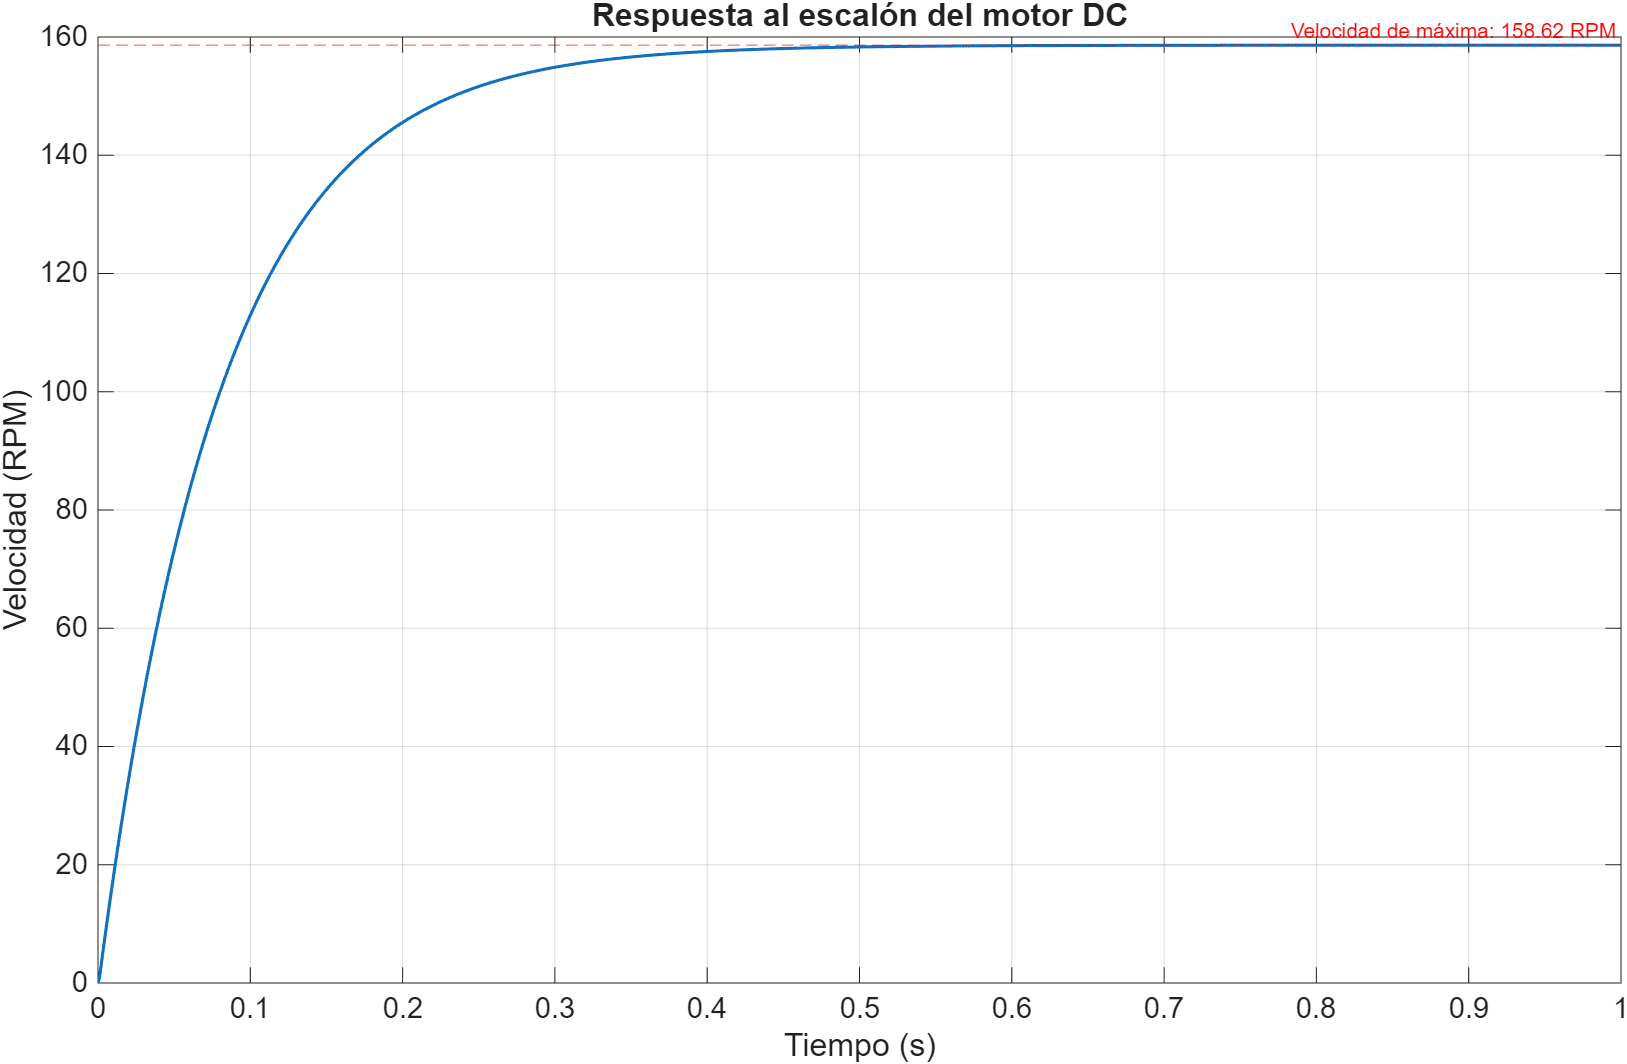
\includegraphics[width=15cm]{Media/matlab_resultado.png}
	\caption{Respuesta al escalón de la velocidad del motor DC obtenida a partir de la respuesta al impulso en MATLAB.}
	\label{fig:resp_escalon}
\end{figure}

A partir de esta respuesta se determinaron los principales parámetros dinámicos del sistema:

\begin{itemize}
	\item Velocidad de estado estable: $\omega_{ss} = 158.62$ RPM
	\item Tiempo de subida: $t_r = 0.176$ s
	\item Tiempo de establecimiento: $t_s = 0.313$ s
\end{itemize}

En la figura \ref{fig:resp_escalon} se observa que el sistema no presenta sobreoscilaciones, lo que indica un comportamiento sobreamortiguado o críticamente amortiguado.

Además, el tiempo de establecimiento es significativamente bajo, lo cual evidencia que el sistema responde rápidamente ante cambios de entrada, siendo adecuado para aplicaciones como el control de velocidad en una puerta corrediza automatizada.



% ====== Referencias ======
\newpage
\printbibliography

\end{document}